\documentclass[12pt, openany, oneside]{book}

\usepackage{listings}
\usepackage[dvipsnames]{xcolor}
\usepackage{ctex}
\usepackage{fontspec}
\usepackage{setspace}
\usepackage{tikz}
\usepackage{anyfontsize}
\usepackage{sectsty}
\usepackage{titlesec}
\usepackage{float}
\usepackage[hidelinks]{hyperref}
\usepackage[a4paper]{geometry}
\usepackage{url}
\usepackage[most]{tcolorbox}
\usepackage{pgf-umlcd}
% \usepackage{minted}

\makeatletter
\newcommand{\verbatimfont}[1]{\renewcommand{\verbatim@font}{\ttfamily#1}}
\makeatother

\usetikzlibrary{calc,trees,positioning,arrows,fit,shapes}
\usetikzlibrary{shapes.multipart,chains}
\usetikzlibrary{automata}

\def\rlwd{.5pt} \def\rlht{2.2ex} \def\rldp{.5ex}
\def\mydiv#1{~%
  \rule[-\rldp]{\rlwd}{\rlht}%
  \setbox0=\hbox{~#1}%
  \stackunder[\dimexpr\rldp-\rlwd]{~#1}{\rule{\wd0}{\rlwd}}%
}

\definecolor{mycolor}{RGB}{0,128,128}
\newtcbox{\mybox} {
    on line,
    colback=mycolor,
    fontupper=\bfseries\color{white},
    boxrule=0pt,
    arc=5pt, 
    boxsep=0pt, 
    left=2pt, 
    right=2pt, 
    top=5pt, 
    bottom=5pt
}

\setstretch{1.5}
\setlength{\parindent}{0cm}

\geometry{a4paper,top=2.5cm,bottom=2.5cm}

\titleformat{\chapter}{\Huge\Huge\bfseries}{\chaptertitlename\ \thechapter{\ }}{0pt}{\Huge}{}
\titlespacing{\chapter}{0pt}{0pt}{12pt}

\definecolor{dkgreen}{rgb}{0,0.4,0}
\definecolor{gray}{rgb}{0.5,0.5,0.5}
\definecolor{mauve}{rgb}{0.58,0,0.82}
\definecolor{LightGray}{gray}{0.9}

\lstset{
    basicstyle=\linespread{1.3} \fontspec{Consolas},    %  the size of the fonts that are used for the code
	basewidth=0.5em,
    numbers=left,            % where to put the line-numbers
    numberstyle=\color{black},  % the style that is used for the line-numbers
    numbersep=10pt,                  % how far the line-numbers are from the code
    backgroundcolor=\color{white},
    showspaces=false,
    showstringspaces=false,
    showtabs=false,
    frame=single,                   % adds a frame around the code
    rulecolor=\color{black},        % if not set, the frame-color may be changed on line-breaks within not-black text (e.g. commens (green here))
    tabsize=4,                      % sets default tabsize to 2 spaces
    captionpos=t,                   % sets the caption-position to bottom
    breaklines=false,                % sets automatic line breaking
    breakatwhitespace=true,        % sets if automatic breaks should only happen at whitespace
    title=\lstname,                   % show the filename of files included with \lstinputlisting;
    % also try caption instead of title
    numberstyle=\color{black},		% line number color
    keywordstyle=\color{blue},          % keyword style
    commentstyle=\color{dkgreen},       % comment style
    stringstyle=\color{mauve},         % string literal style
    escapeinside={\%*}{*)},            % if you want to add LaTeX within your code
    morekeywords={*,...}               % if you want to add more keywords to the set
}

\begin{document}

\thispagestyle{empty}

\begin{tikzpicture}[overlay,remember picture]
	% Background color
	\fill[
		black!2]
	(current page.south west) rectangle (current page.north east);

	% Rectangles
	\shade[
		left color=Dandelion,
		right color=Dandelion!40,
		transform canvas ={rotate around ={45:($(current page.north west)+(0,-6)$)}}]
	($(current page.north west)+(0,-6)$) rectangle ++(9,1.5);

	\shade[
		left color=lightgray,
		right color=lightgray!50,
		rounded corners=0.75cm,
		transform canvas ={rotate around ={45:($(current page.north west)+(.5,-10)$)}}]
	($(current page.north west)+(0.5,-10)$) rectangle ++(15,1.5);

	\shade[
		left color=lightgray,
		rounded corners=0.3cm,
		transform canvas ={rotate around ={45:($(current page.north west)+(.5,-10)$)}}] ($(current page.north west)+(1.5,-9.55)$) rectangle ++(7,.6);

	\shade[
		left color=orange!80,
		right color=orange!60,
		rounded corners=0.4cm,
		transform canvas ={rotate around ={45:($(current page.north)+(-1.5,-3)$)}}]
	($(current page.north)+(-1.5,-3)$) rectangle ++(9,0.8);

	\shade[
		left color=red!80,
		right color=red!80,
		rounded corners=0.9cm,
		transform canvas ={rotate around ={45:($(current page.north)+(-3,-8)$)}}] ($(current page.north)+(-3,-8)$) rectangle ++(15,1.8);

	\shade[
		left color=orange,
		right color=Dandelion,
		rounded corners=0.9cm,
		transform canvas ={rotate around ={45:($(current page.north west)+(4,-15.5)$)}}]
	($(current page.north west)+(4,-15.5)$) rectangle ++(30,1.8);

	\shade[
		left color=RoyalBlue,
		right color=Emerald,
		rounded corners=0.75cm,
		transform canvas ={rotate around ={45:($(current page.north west)+(13,-10)$)}}]
	($(current page.north west)+(13,-10)$) rectangle ++(15,1.5);

	\shade[
		left color=lightgray,
		rounded corners=0.3cm,
		transform canvas ={rotate around ={45:($(current page.north west)+(18,-8)$)}}]
	($(current page.north west)+(18,-8)$) rectangle ++(15,0.6);

	\shade[
		left color=lightgray,
		rounded corners=0.4cm,
		transform canvas ={rotate around ={45:($(current page.north west)+(19,-5.65)$)}}]
	($(current page.north west)+(19,-5.65)$) rectangle ++(15,0.8);

	\shade[
		left color=OrangeRed,
		right color=red!80,
		rounded corners=0.6cm,
		transform canvas ={rotate around ={45:($(current page.north west)+(20,-9)$)}}]
	($(current page.north west)+(20,-9)$) rectangle ++(14,1.2);

	% Year
	% \draw[ultra thick,gray]
	% ($(current page.center)+(5,2)$) -- ++(0,-3cm)
	node[
			midway,
			left=0.25cm,
			text width=5cm,
			align=right,
			black!75
		]
		{
			% {\fontsize{25}{30} \selectfont \bf ANNUAL \\[10pt] REPORT}
		}
	node[
			midway,
			right=0.25cm,
			text width=6cm,
			align=left,
			orange]
		{
			% {\fontsize{72}{86.4} \selectfont 2020}
		};

	% Title
	\node[align=center] at ($(current page.center)+(0,-6)$)
	{
	{\fontsize{64}{64} \selectfont {{C++面向对象}}} \\[2cm]
	{\fontsize{20}{19.2} \selectfont \textcolor{orange}{ \bf 极夜酱}} \\[4pt]
	};
\end{tikzpicture}

\newpage

\pagestyle{plain}
\setcounter{page}{1}
\setcounter{tocdepth}{1}
\tableofcontents

\newpage

\setcounter{page}{1}

% \chapter{Hello World!}

\section{Hello World!}

\subsection{编程语言(Programming Language)}

程序是为了让计算机去解决某些问题,它由一系列指令构成。但是计算机并不能理解人类的语言,即使是最简单的,例如“计算一下1+2是多少”。\\

计算机采用的是二进制(binary),也就是只能够理解0和1,因此编程语言用于作为人类与计算机之间沟通的桥梁。

\begin{figure}[H]
	\centering
	\includegraphics[scale=0.9]{img/Chapter1/1-1/1.png}
\end{figure}

通过使用编程语言来描述解决问题的步骤,从而让计算机一步一步去执行。流程图(flow chat)成为了一种程序的图形化表示方式。\\

\begin{figure}[H]
	\centering
	\begin{tikzpicture}[node distance=2cm]
		\node (start) [startend] {Start};
		\node (init) [io, below of=start] {$ i = 0 $, $ sum = 0 $};
		\node (decision)  [decision, below of=init] {$ i \le 100 $?};
		\node (accumulation) [process, below of=decision] {$ sum = sum + i $};
		\node (update) [process, below of=accumulation] {$ i = i + 1 $};
		\node (output) [io, right of=decision, xshift=2.5cm] {print $ sum $};
		\node (end) [startend, below of=update] {End};

		\draw [arrow] (start) -- (init);
		\draw [arrow] (init) -- (decision);
		\draw [arrow] (decision) -- node[anchor=east] {yes } (accumulation);
		\draw [arrow] (accumulation) -- (update);
		\draw [arrow] (update) -- (-3,-8) -- (-3,-4) -- (decision);
		\draw [arrow] (decision) -- node[anchor=south] {no} (output);
		\draw [arrow] (output) |- (end);
	\end{tikzpicture}
	\caption{计算$ \sum_{i=1}^{100} i $的流程图}
\end{figure}

\vspace{0.5cm}

\subsection{Hello World!}

Hello World是学习编程的第一个程序,它的作用是向屏幕输出"Hello World!"。\\

\mybox{Hello World!}

\begin{lstlisting}[language=C++]
#include <iostream>

using namespace std;

int main()
{
	cout << "Hello World!" << endl;
	return 0;
}
\end{lstlisting}

\begin{tcolorbox}
	\mybox{运行结果}
	\begin{verbatim}
Hello World!
	\end{verbatim}
\end{tcolorbox}

\#include <iostream>用于包含输入输出库的头文件(header file),这样才能够在程序中进行输入输出相关的操作。\\

using namespace std表示使用std命名空间。\\

main()是程序的入口,程序运行后会首先执行main()中的代码。cout的功能是在屏幕上输出数据,endl表示输出一个换行符。最后的分号用于表示一条语句的结束,注意不要使用中文的分号。\\

return 0表示main()运行结束,返回值为0,一般返回0用于表示程序正常结束。\\

不同编程语言的Hello World写法大同小异,可以看出编程语言的基本结构是相似的。\\

\mybox{C}

\begin{lstlisting}[language=C]
#include <stdio.h>

int main() {
	printf("Hello World!\n");
	return 0;
}
\end{lstlisting}

\vspace{0.5cm}

\mybox{Java}

\begin{lstlisting}[language=Java]
public class HelloWorld {
    public static void main(String[] args) {
        System.out.println("Hello World!");
    }
}
\end{lstlisting}

\vspace{0.5cm}

\mybox{Python}

\begin{lstlisting}[language=Python]
print("Hello World!")
\end{lstlisting}

\vspace{0.5cm}

\subsection{注释(Comment)}

注释就是对代码的解释和说明,它并不会程序所执行。注释能提高程序的可读性,让人更加容易了解代码的功能。\\

注释一般分为单行注释和多行注释:

\begin{enumerate}
	\item 单行注释:以//开头,该行之后的内容视为注释。
	\item 多行注释:以/*开头,*/结束,中间的内容视为注释。
\end{enumerate}

\vspace{0.5cm}

\mybox{注释}

\begin{lstlisting}[language=C++]
/*
* Author: Terry
* Date: 2022/11/16
*/

#include <iostream>      // header file

using namespace std;

int main()
{
	cout << "Hello World!" << endl;
	return 0;
}
\end{lstlisting}

\newpage

\section{数据类型}

\subsection{数据类型(Data Types)}

在计算机中,每个数据一般都有一个对应的类型,基础数据类型包括:

\begin{enumerate}
	\item 整型
	      \begin{itemize}
		      \item 短整型short
		      \item 整型int
		      \item 长整型long
		      \item 长长整型long long
	      \end{itemize}

	\item 浮点型
	      \begin{itemize}
		      \item 单精度浮点数float
		      \item 双精度浮点数double
	      \end{itemize}

	\item 字符型char
\end{enumerate}

\vspace{0.5cm}

不同的数据类型所占的内存空间大小不同,因此所能表示的数值范围也不同。\\

\begin{table}[H]
	\centering
	\setlength{\tabcolsep}{5mm}{
		\begin{tabular}{|c|c|c|}
			\hline
			\textbf{数据类型} & \textbf{大小} & \textbf{取值范围}           \\
			\hline
			short             & 2字节         & $ -2^{15} \sim 2^{15} - 1 $ \\
			\hline
			int               & 4字节         & $ -2^{31} \sim 2^{31} - 1 $ \\
			\hline
			long              & 4字节         & $ -2^{31} \sim 2^{31} - 1 $ \\
			\hline
			long long         & 8字节         & $ -2^{63} \sim 2^{63} - 1 $ \\
			\hline
			float             & 4字节         & 7位有效数字                 \\
			\hline
			double            & 8字节         & 15位有效数字                \\
			\hline
			char              & 1字节         & $ -128 \sim 127 $           \\
			\hline
		\end{tabular}
	}
\end{table}

\vspace{0.5cm}

\subsection{变量(Variable)}

变量是用来存储数据的内存空间,每个变量都有一个类型,变量中只能存储对应类型的数据。

\vspace{-0.5cm}

\begin{lstlisting}[language=C++]
int num = 10;
double salary = 8232.56;
\end{lstlisting}

\vspace{0.5cm}

变量的命名需要符合规范:

\begin{enumerate}
	\item 由字母、数字和下划线组成,不能以数字开头
	\item 不可以使用编程语言中预留的关键字
	\item 使用英语单词,顾名思义
\end{enumerate}

关键字是编程语言内置的一些名称,具有特殊的用处和意义,因此不应该作为变量名,防止产生歧义。\\

\begin{table}[H]
	\centering
	\setlength{\tabcolsep}{5mm}{
		\begin{tabular}{|c|c|c|c|c|}
			\hline
			asm      & auto     & break     & case     & catch    \\
			\hline
			char     & class    & const     & continue & default  \\
			\hline
			delete   & do       & double    & else     & enum     \\
			\hline
			extern   & float    & for       & friend   & goto     \\
			\hline
			if       & inline   & int       & long     & new      \\
			\hline
			operator & private  & protected & public   & register \\
			\hline
			return   & short    & signed    & sizeof   & static   \\
			\hline
			struct   & switch   & template  & this     & throw    \\
			\hline
			try      & typedef  & union     & unsigned & virtual  \\
			\hline
			void     & volatile & while     &          &          \\
			\hline
		\end{tabular}
	}
	\caption{关键字}
\end{table}

\vspace{0.5cm}

\subsection{常量(Constant)}

变量的值在程序运行过程中可以修改,但有一些数据的值是固定的,为了防止这些数据被随意改动,可以将这些数据定义为常量。\\

在数据类型前加上const关键字,即可定义常量,常量一般使用大写表示。如果在程序中尝试修改常量,将会报错。\\

\mybox{常量}

\begin{lstlisting}[language=C++]
#include <iostream>

using namespace std;

int main()
{
	const double PI = 3.1415;
	PI = 4;
	return 0;
}
\end{lstlisting}

\begin{tcolorbox}
	\mybox{运行结果}\\
	\textcolor{red}{error: assignment of read-only variable "PI"}
\end{tcolorbox}

\newpage

\section{输入输出}

\subsection{cout}

cout是输出流对象,用来向屏幕输出数据。但是有些需要输出的字符在编程语言中具有特殊含义,因此这些特殊的字符,需要经过转义后输出。\\

\begin{table}[H]
	\centering
	\setlength{\tabcolsep}{5mm}{
		\begin{tabular}{|c|c|}
			\hline
			\textbf{转义字符}      & \textbf{描述}                \\
			\hline
			\lstinline|\\| & 反斜杠\lstinline|\| \\
			\hline
			\lstinline|\'| & 单引号\lstinline|'| \\
			\hline
			\lstinline|\"| & 双引号\lstinline|"| \\
			\hline
			\lstinline|\n| & 换行                         \\
			\hline
			\lstinline|\t| & 制表符                       \\
			\hline
		\end{tabular}
	}
	\caption{转义字符}
\end{table}

\mybox{转义字符}

\begin{lstlisting}[language=C++]
#include <iostream>

using namespace std;

int main()
{
	cout << "\"Hello\nWorld\"" << endl;
	return 0;
}
\end{lstlisting}

\begin{tcolorbox}
	\mybox{运行结果}
	\begin{verbatim}
"Hello
World"
	\end{verbatim}
\end{tcolorbox}

在对变量的值进行输出时,可以使用格式控制符改变输出的格式。\\

\mybox{长方形面积}

\begin{lstlisting}[language=C++]
#include <iostream>
#include <iomanip>

using namespace std;

int main()
{
	int length = 10;
	int width = 5;
	double area = length * width;

	cout << "Area = " << length << " * " << width << " = "
			<< fixed << setprecision(2) << area << endl;
	return 0;
}
\end{lstlisting}

\begin{tcolorbox}
	\mybox{运行结果}
	\begin{verbatim}
Area = 10 * 5 = 50.00
	\end{verbatim}
\end{tcolorbox}

\vspace{0.5cm}

\subsection{printf()}

printf()是C语言中的输出函数,包含在头文件<cstdio>中,用于向屏幕输出指定格式的文本,使用对应类型的占位符可以更加方便地输出变量的值。\\

\begin{table}[H]
	\centering
	\setlength{\tabcolsep}{5mm}{
		\begin{tabular}{|c|c|}
			\hline
			\textbf{数据类型} & \textbf{占位符} \\
			\hline
			int               & \%d             \\
			\hline
			float             & \%f             \\
			\hline
			double            & \%f             \\
			\hline
			char              & \%c             \\
			\hline
		\end{tabular}
	}
	\caption{占位符}
\end{table}

\vspace{-0.5cm}

\begin{lstlisting}[language=C]
printf("Area = %d * %d = %.2f\n", length, width, area);
\end{lstlisting}

\vspace{0.5cm}

\subsection{cin}

有时候一些数据需要从键盘输入,cin可以读取对应类型的数据,并赋值给相应的变量。\\

在使用cin前,通常会使用cout先输出一句提示信息,告诉用户需要输入什么数据。\\

\mybox{圆面积}

\begin{lstlisting}[language=C++]
#include <iostream>
#include <cmath>
#include <iomanip>

using namespace std;

int main()
{
	const double PI = 3.14159;
	double r;
	double area;

	cout << "Radius: ";
	cin >> r;

	area = PI * pow(r, 2);
	cout << "Area = " << fixed << setprecision(2) << area << endl;
	
	return 0;
}
\end{lstlisting}

\begin{tcolorbox}
	\mybox{运行结果}
	\begin{verbatim}
Radius: 5
Area = 78.54
	\end{verbatim}
\end{tcolorbox}

头文件<cmath>中定义了一些常用的数学函数,例如pow(x, y)可用于计算$ x $的$ y $次方。\\

\newpage

\section{表达式}

\subsection{算术运算符}

大部分编程语言中的除法与数学中的除法意义不同。\\

当相除的两个数都为整数时,那么就会进行整除运算,因此结果仍为整数,例如21 / 4 = 5。\\

如果相除的两个数中至少有一个为浮点数时,那么就会进行普通的除法运算,结果为浮点数,例如21.0 / 4 = 5.25。\\

取模(modulo)运算符\%用于计算两个整数相除之后的余数,例如22 \% 3 = 1、4 \% 7 = 4。\\

\mybox{逆序三位数}

\begin{lstlisting}[language=C++]
#include <iostream>

using namespace std;

int main()
{
	int num;
	int a, b, c;

	cout << "Enter a 3-digit integer: ";
	cin >> num;

	a = num / 100;
	b = num / 10 % 10;
	c = num % 10;

	cout << "Reversed: " << c*100 + b*10 + a << endl;
	return 0;
}
\end{lstlisting}

\begin{tcolorbox}
	\mybox{运行结果}
	\begin{verbatim}
Enter a 3-digit integer: 520
Reversed: 25
	\end{verbatim}
\end{tcolorbox}

\vspace{0.5cm}

\subsection{复合运算符}

使用复合运算符可以使表达式更加简洁。例如\lstinline|a = a + b|可以写成\lstinline|a += b|,-=、*=、/=、\%=等复合运算符的使用方式同理。\\

当需要给一个变量的值加/减1时,除了可以使用\lstinline|a += 1|或\lstinline|a -= 1|之外,还可以使用++或--运算符,但是\lstinline|++|和\lstinline|--|可以出现在变量之前或之后:\\

\begin{table}[H]
	\centering
	\setlength{\tabcolsep}{5mm}{
		\begin{tabular}{|c|l|}
			\hline
			\textbf{表达式}         & \textbf{含义}         \\
			\hline
			\lstinline|a++| & 执行完所在语句后自增1 \\
			\hline
			\lstinline|++a| & 在执行所在语句前自增1 \\
			\hline
			\lstinline|a--| & 执行完所在语句后自减1 \\
			\hline
			\lstinline|--a| & 在执行所在语句前自减1 \\
			\hline
		\end{tabular}
	}
	\caption{自增/自减运算符}
\end{table}

\mybox{自增/自减运算符}

\begin{lstlisting}[language=C++]
#include <iostream>

using namespace std;

int main()
{
	int n = 10;

	cout << n++ << endl;
	cout << ++n << endl;
	cout << n-- << endl;
	cout << --n << endl;

	return 0;
}
\end{lstlisting}

\begin{tcolorbox}
	\mybox{运行结果}
	\begin{verbatim}
10
12
12
10
	\end{verbatim}
\end{tcolorbox}

\vspace{0.5cm}

\subsection{隐式类型转换}

在计算机计算的过程中,只有类型相同的数据才可以进行运算。例如整数+整数、浮点数/浮点数等。\\

但是很多时候,我们仍然可以对不同类型的数据进行运算,而并不会产生错误,例如整数+浮点数。这是由于编译器会自动进行类型转换。在整数+浮点数的例子中,编译器会将整数转换为浮点数,这样就可以进行运算了。\\

编译器选择将整数转换为浮点数,而不是将浮点数转换为整数的原因在于,浮点数相比整数能够表示的范围更大。例如整数8可以使用8.0表示,而浮点数9.28变为整数9后就会丢失精度。\\

隐式类型转换最常见的情形就是除法运算,这也是导致整数/整数=整数、整数/浮点数=浮点数的原因。\\

\subsection{显式类型转换}

有些时候编译器无法自动进行类型转换,这时就需要我们手动地强制类型转换。\\

\mybox{显式类型转换}

\begin{lstlisting}[language=C++]
#include <iostream>
#include <iomanip>

using namespace std;

int main()
{
	int total = 821;
	int num = 10;
	double average = (double)total / num;
	cout << "Average = " << fixed << setprecision(2) << average << endl;
	return 0;
}
\end{lstlisting}

\begin{tcolorbox}
	\mybox{运行结果}
	\begin{verbatim}
Average = 82.10
	\end{verbatim}
\end{tcolorbox}

\newpage
% \chapter{分支}

\section{逻辑运算符}

\subsection{关系运算符}

编程中经常需要使用关系运算符来比较两个数据的大小,比较的结果是一个布尔值(boolean),即True(非0)或False(0)。\\

在编程中需要注意,一个等号=表示赋值运算,而两个等号==表示比较运算。\\

\begin{table}[H]
	\centering
	\setlength{\tabcolsep}{5mm}{
		\begin{tabular}{|c|c|}
			\hline
			\textbf{数学符号} & \textbf{关系运算符} \\
			\hline
			$ < $             & <                   \\
			\hline
			$ > $             & >                   \\
			\hline
			$ \le $           & <=                  \\
			\hline
			$ \ge $           & >=                  \\
			\hline
			$ = $             & ==                  \\
			\hline
			$ \ne $           & !=                  \\
			\hline
		\end{tabular}
	}
\end{table}

\vspace{0.5cm}

\subsection{逻辑运算符}

逻辑运算符用于连接多个关系表达式,其结果也是一个布尔值。\\

\begin{enumerate}
	\item 逻辑与\&\&:当多个条件全部为True,结果为True。\\
	      \begin{table}[H]
		      \centering
		      \setlength{\tabcolsep}{5mm}{
			      \begin{tabular}{|c|c|c|}
				      \hline
				      \textbf{条件1} & \textbf{条件2} & \textbf{条件1 \&\& 条件2} \\
				      \hline
				      T              & T              & T                         \\
				      \hline
				      T              & F              & F                         \\
				      \hline
				      F              & T              & F                         \\
				      \hline
				      F              & F              & F                         \\
				      \hline
			      \end{tabular}
		      }
	      \end{table}

	\item 逻辑或||:多个条件至少有一个为True时,结果为True。\\
	      \begin{table}[H]
		      \centering
		      \setlength{\tabcolsep}{5mm}{
			      \begin{tabular}{|c|c|c|}
				      \hline
				      \textbf{条件1} & \textbf{条件2} & \textbf{条件1 || 条件2} \\
				      \hline
				      T              & T              & T                       \\
				      \hline
				      T              & F              & T                       \\
				      \hline
				      F              & T              & T                       \\
				      \hline
				      F              & F              & F                       \\
				      \hline
			      \end{tabular}
		      }
	      \end{table}

	\item 逻辑非!:条件为True时,结果为False;条件为False时,结果为True。\\
	      \begin{table}[H]
		      \centering
		      \setlength{\tabcolsep}{5mm}{
			      \begin{tabular}{|c|c|}
				      \hline
				      \textbf{条件} & \textbf{!条件} \\
				      \hline
				      T             & F              \\
				      \hline
				      F             & T              \\
				      \hline
			      \end{tabular}
		      }
	      \end{table}
\end{enumerate}

\newpage

\section{if}

\subsection{if}

if语句用于判断一个条件是否成立,如果成立则进入语句块,否则不执行。\\

\mybox{年龄}

\begin{lstlisting}[language=C++]
#include <iostream>

using namespace std;

int main()
{
	int age;
	cout << "Enter your age: ";
	cin >> age;
	if(age > 0 && age < 18)
	{
		cout << "Minor" << endl;
	}
	return 0;
}
\end{lstlisting}

\begin{tcolorbox}
	\mybox{运行结果}
	\begin{verbatim}
Enter your age: 17
Minor
\end{verbatim}
\end{tcolorbox}

\vspace{0.5cm}

\subsection{if-else}

if-else的结构与if类似,只是在if语句块中的条件不成立时,执行else语句块中的语句。\\

\mybox{闰年}

\begin{lstlisting}[language=C++]
#include <iostream>

using namespace std;

int main()
{
	int year;
	cout << "Enter a year: ";
	cin >> year;

	/*
		* A year is a leap year if it is
		* 1. exactly divisible by 4, and not divisible by 100;
		* 2. or is exactly divisible by 400
		*/
	if((year % 4 == 0 && year % 100 != 0) || year % 400 == 0)
	{
		cout << "Leap year" << endl;
	}
	else
	{
		cout << "Common year" << endl;
	}

	return 0;
}
\end{lstlisting}

\begin{tcolorbox}
	\mybox{运行结果}
	\begin{verbatim}
Enter a year: 2020
Leap year
\end{verbatim}
\end{tcolorbox}

\vspace{0.5cm}

\subsection{if-else if-else}

当需要对更多的条件进行判断时,可以使用if-else if-else语句。\\

\mybox{字符}

\begin{lstlisting}[language=C++]
#include <iostream>

using namespace std;

int main()
{
	char c;
	cout << "Enter a character: ";
	cin >> c;

	if(c >= 'a' && c <= 'z')
	{
		printf("Lowercase\n");
	}
	else if(c >= 'A' && c <= 'Z')
	{
		printf("Uppercase\n");
	}
	else if(c >= '0' && c <= '9')
	{
		printf("Digit\n");
	}
	else
	{
		printf("Special character\n");
	}
	
	return 0;
}
\end{lstlisting}

\begin{tcolorbox}
	\mybox{运行结果}
	\begin{verbatim}
Enter a character: T
Uppercase
\end{verbatim}
\end{tcolorbox}

\newpage

\section{switch}

\subsection{switch}

switch结构用于根据一个整数值,选择对应的case执行。需要注意的是,当对应的case中的代码被执行完后,并不会像if语句一样跳出switch结构,而是会继续向后执行,直到遇到break。\\

\mybox{计算器}

\begin{lstlisting}[language=C++]
#include <iostream>

using namespace std;

int main() {
	int num1, num2;
	char op;

	cout << "Enter an expression: ";
	cin >> num1 >> op >> num2;

	switch (op)
	{
	case '+':
		cout << num1 << " + " << num2 << " = " << num1 + num2 << endl;
		break;
	case '-':
		cout << num1 << " - " << num2 << " = " << num1 - num2 << endl;
		break;
	case '*':
		cout << num1 << " * " << num2 << " = " << num1 * num2 << endl;
		break;
	case '/':
		cout << num1 << " / " << num2 << " = " << num1 / num2 << endl;
		break;
	default:
		cout << "Error! Operator is not supported" << endl;
		break;
	}

	return 0;
}
\end{lstlisting}

\begin{tcolorbox}
	\mybox{运行结果}
	\begin{verbatim}
Enter an expression: 5 * 8
5 * 8 = 40
\end{verbatim}
\end{tcolorbox}

\newpage
% \chapter{继承}

\section{继承}

\subsection{继承(Inheritance)}

继承是面向对象的三大特征之一,程序中的继承是类与类之间的特征和行为的一种赠予或获取。两个类之间的继承必须满足“is a”的关系。子类继承自父类,父类也称基类或超类,子类也称派生类。 \\

\begin{figure}[H]
	\centering
	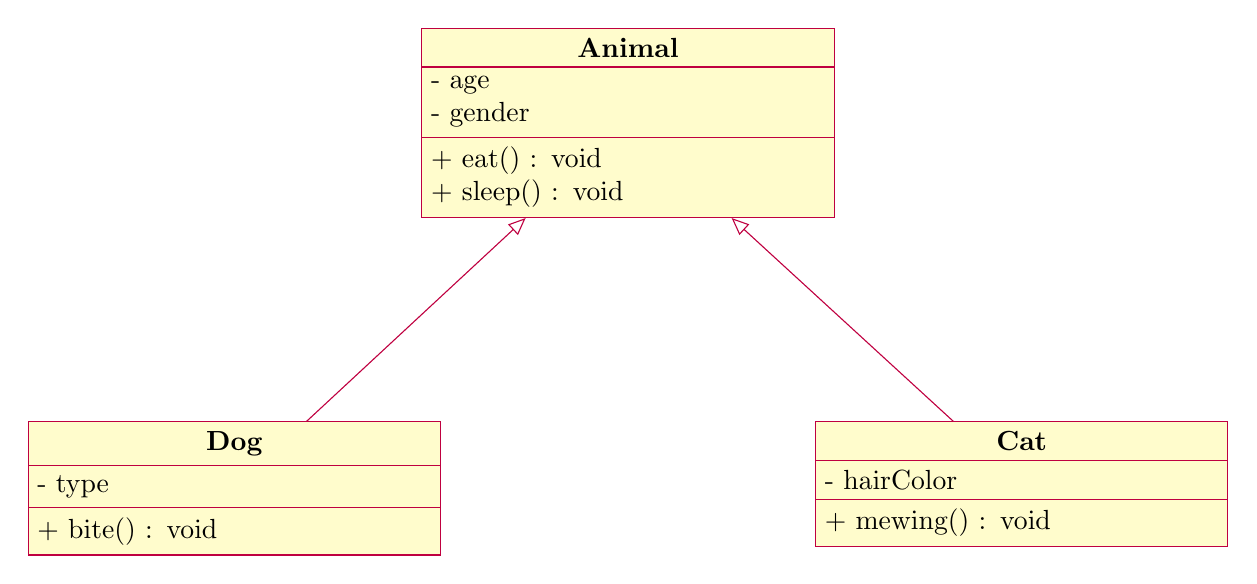
\begin{tikzpicture}
		\begin{class}{Animal}{0,0}
			\attribute{- age}
			\attribute{- gender}
			\operation{+ eat() : void}
			\operation{+ sleep() : void}
		\end{class}

		\begin{class}{Dog}{-5,-5}
			\inherit{Animal}
			\attribute{- type}
			\operation{+ bite() : void}
		\end{class}

		\begin{class}{Cat}{5,-5}
			\inherit{Animal}
			\attribute{- hairColor}
			\operation{+ mewing() : void}
		\end{class}
	\end{tikzpicture}
	\caption{继承}
\end{figure}

产生继承关系后,子类可以使用父类中的属性和方法,也可以定义子类独有的属性和方法。

\vspace{-0.5cm}

\begin{lstlisting}[language=Java]
class subclass : access_modifier superclass {
    // code
};
\end{lstlisting}

继承时通常使用public类型。当一个类public继承于父类时,父类的public成员也是子类的public成员,父类的protected成员也是子类的protected成员,父类的private成员不能被继承。 \\

继承的好处是可以提高代码的复用性、提高代码的拓展性。 \\

\mybox{继承}

\begin{lstlisting}[language=C++, title=animal.h]
#ifndef _ANIMAL_H_
#define _ANIMAL_H_

#include <string>

class Animal {
public:
    Animal(std::string name = "", int age = 0);
    void eat();

private:
    std::string name;
    int age;
};

#endif
\end{lstlisting}

\begin{lstlisting}[language=C++, title=animal.cpp]
#include "animal.h"
#include <iostream>

using namespace std;

Animal::Animal(string name, int age)
    : name(name), age(age) {}

void Animal::eat() {
    cout << "eating" << endl;
}
\end{lstlisting}

\begin{lstlisting}[language=C++, title=dog.h]
#ifndef _DOG_H
#define _DOG_H_

#include "animal.h"
#include <string>

class Dog : public Animal {
public:
    Dog(std::string name, int age, std::string type = "");
    void bite();
    
private:
    std::string type;
};

#endif
\end{lstlisting}

\begin{lstlisting}[language=C++, title=dog.cpp]
#include "dog.h"
#include <iostream>

using namespace std;

Dog::Dog(string name, int age, string type)
    : Animal(name, age), type(type) {}

void Dog::bite() {
    cout << "biting" << endl;
}
\end{lstlisting}

\begin{lstlisting}[language=C++, title=test\_dog.cpp]
#include <iostream>
#include "dog.h"

using namespace std;

int main() {
    Dog dog("狗子", 3, "哈士奇");
    dog.eat();
    dog.bite();
    return 0;
}
\end{lstlisting}

\begin{tcolorbox}
	\mybox{运行结果}
	\begin{verbatim}
eating
biting
	\end{verbatim}
\end{tcolorbox}

\newpage

\section{多继承}

\subsection{多继承}

C++支持多继承,即一个子类可以有两个或更多个父类。多继承时通过使用逗号将多个父类隔开,每个父类都可以用不同访问限定符修饰。 \\

当多个父类中有同名的成员时,就会产生命名冲突,因此这时就需要在成员前加上类名和域限定符【::】消除二义性。 \\

\mybox{多继承}

\begin{lstlisting}[language=C++, title=date.h]
#ifndef _DATE_H_
#define _DATE_H_

#include <string>

class Date {
public:
    Date(int year = 1970, int month = 1, int day = 1);
    std::string getDate();

private:
    int year;
    int month;
    int day;
};

#endif
\end{lstlisting}

\begin{lstlisting}[language=C++, title=date.cpp]
#include "date.h"

using namespace std;

Date::Date(int year, int month, int day)
    : year(year), month(month), day(day) {}

string Date::getDate() {
    char format[128];
    snprintf(format, sizeof(format), 
            "%04d/%02d/%02d", year, month, day);
    string dateStr(format);
    return dateStr;
}
\end{lstlisting}

\begin{lstlisting}[language=C++, title=time.h]
#ifndef _TIME_H_
#define _TIME_H_

#include <string>

class Time {
public:
    Time(int hour = 0, int minute = 0, int second = 0);
    std::string getTime();

private:
    int hour;
    int minute;
    int second;
};

#endif
\end{lstlisting}

\begin{lstlisting}[language=C++, title=time.cpp]
#include "time.h"

using namespace std;

Time::Time(int hour, int minute, int second)
    : hour(hour), minute(minute), second(second) {}

string Time::getTime() {
    char format[128];
    snprintf(format, sizeof(format), 
            "%02d:%02d:%02d", hour, minute, second);
    string timeStr(format);
    return timeStr;
}
\end{lstlisting}

\begin{lstlisting}[language=C++, title=date\_time.h]
#ifndef _DATE_TIME_H_
#define _DATE_TIME_H_

#include "date.h"
#include "time.h"
#include <string>

class DateTime : public Date, public Time {
public:
    DateTime(int year = 1970, int month = 1, int day = 1,
             int hour = 0, int minute = 0, int second = 0);
    std::string getDateTime();

private:
    int year;
    int month;
    int day;
    int hour;
    int minute;
    int second;
};

#endif
\end{lstlisting}

\begin{lstlisting}[language=C++, title=date\_time.cpp]
#include "date_time.h"

using namespace std;

DateTime::DateTime(int year, int month, int day,
         int hour, int minute, int second)
  : Date(year, month, day),
    Time(hour, minute, second) {}

string DateTime::getDateTime() {
    return getDate() + " " + getTime();
}
\end{lstlisting}

\begin{lstlisting}[language=C++, title=test\_date\_time.cpp]
#include <iostream>
#include "date_time.h"

using namespace std;

int main() {
    DateTime dt1;
    cout << dt1.getDateTime() << endl;
    DateTime dt2(2021, 8, 31, 13, 50, 23);
    cout << dt2.getDateTime() << endl;
    return 0;
}
\end{lstlisting}

\begin{tcolorbox}
	\mybox{运行结果}
	\begin{verbatim}
1970/01/01 00:00:00
2021/08/31 13:50:23
	\end{verbatim}
\end{tcolorbox}

\newpage

\section{向上转型与向下转型}

\subsection{向上转型 / 向下转型}

对象由子类类型转型为父类类型,即是向上转型。向上转型是一种隐式转换,一定会转型成功。向上转型后的对象,只能访问父类中定义的成员。 \\

由父类类型转型转型为子类类型,即是向下转型。向下转型是不安全的,可能会导致数据的丢失,原因是父类的指针或引用中可能不包含子类成员的内存。 \\

\mybox{向上转型}

\begin{lstlisting}[language=C++, title=animal.h]
#ifndef _ANIMAL_H_
#define _ANIMAL_H_

#include <string>

class Animal {
public:
    Animal(std::string name = "");
    std::string getName();

private:
    std::string name;
};

#endif
\end{lstlisting}

\begin{lstlisting}[language=C++, title=animal.cpp]
#include "animal.h"

using namespace std;

Animal::Animal(string name) : name(name) {}

string Animal::getName() {
    return name;
}
\end{lstlisting}

\begin{lstlisting}[language=C++, title=dog.h]
#ifndef _DOG_H_
#define _DOG_H_

#include "animal.h"
#include <string>

class Dog : public Animal {
public:
    Dog(std::string name, std::string type = "");
    std::string getType();

private:
    std::string type;
};

#endif
\end{lstlisting}

\begin{lstlisting}[language=C++, title=dog.cpp]
#include "dog.h"

using namespace std;

Dog::Dog(string name, string type) 
    : Animal(name), type(type) {}

string Dog::getType() {
    return type;
}
\end{lstlisting}

\begin{lstlisting}[language=C++, title=test\_dog.cpp]
#include <iostream>
#include "animal.h"
#include "dog.h"

using namespace std;

int main() {
    Dog dog("狗子", "哈士奇");
    cout << "dog: " << dog.getName()
         << ", " << dog.getType() << endl; 

    Animal animal = (Animal)dog;
    cout << "animal: " << animal.getName() << endl;
    return 0;
}
\end{lstlisting}

\begin{tcolorbox}
	\mybox{运行结果}
	\begin{verbatim}
dog: 狗子, 哈士奇
animal: 狗子
    \end{verbatim}
\end{tcolorbox}

\newpage
\chapter{数组}

\section{数组}

\subsection{数组(Array)}

数组能够存储一组类型相同的元素,数组在声明时必须指定它的大小(容量),数组的大小是固定的,无法在运行时动态改变。数组通过下标(index)来访问某一位置上的元素,下标从0开始。

\vspace{-0.5cm}

\begin{lstlisting}[language=C]
int arr[5] = {3, 6, 8, 2, 4};
\end{lstlisting}

\begin{figure}[H]
	\centering
	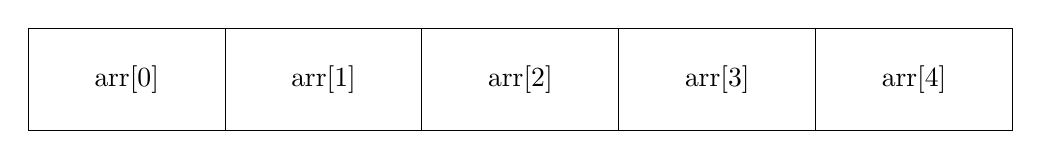
\begin{tikzpicture}[scale=0.5]
		\draw[-] (0,0) -- (5,0) -- (10,0) -- (15,0) -- (20,0) -- (25,0) -- (25,2.6) -- (20,2.6) -- (15,2.6) -- (10,2.6) -- (5,2.6) -- (0,2.6) -- (0,0);
		\draw[-] (5,0) -- (5,2.6);
		\draw[-] (10,0) -- (10,2.6);
		\draw[-] (15,0) -- (15,2.6);
		\draw[-] (20,0) -- (20,2.6);

		\draw (2.5,1.3) node {arr[0]};
		\draw (7.5,1.3) node {arr[1]};
		\draw (12.5,1.3) node {arr[2]};
		\draw (17.5,1.3) node {arr[3]};
		\draw (22.5,1.3) node {arr[4]};
	\end{tikzpicture}
\end{figure}

如果在声明数组时没有指定数组的大小,那么将根据初始化的元素个数来确定。

\vspace{-0.5cm}

\begin{lstlisting}[language=C]
int arr[] = {3, 6, 8, 2, 4, 0, 1, 7};
\end{lstlisting}

通过下标可以访问数组中的元素,下标的有效范围是0 $ \sim $ 数组的长度 - 1,如果使用不合法的下标就会导致数组越界。

\vspace{-0.5cm}

\begin{lstlisting}[language=C]
printf("%d\n", arr[0]);		// 3
printf("%d\n", arr[3]);		// 2
printf("%d\n", arr[7]);		// 7
\end{lstlisting}

当数组的容量比较大时,可以使用循环来初始化数组。

\vspace{-0.5cm}

\begin{lstlisting}[language=C]
int arr[10];

for(int i = 0; i < 10; i++) {
	arr[i] = i + 1;
}
\end{lstlisting}

\vspace{0.5cm}

\mybox{查找数据}

\begin{lstlisting}[language=C]
#include <stdio.h>
#include <stdbool.h>

int main() {
	int n;
	printf("Enter the number of elements: ");
	scanf("%d", &n);

	int arr[n];
	printf("Enter the elements: ");
	for (int i = 0; i < n; i++) {
		scanf("%d", &arr[i]);
	}

	int key;
	printf("Enter the key: ");
	scanf("%d", &key);

	bool found = false;
	for (int i = 0; i < n; i++) {
		if (arr[i] == key) {
			found = true;
			break;
		}
	}

	if (found) {
		printf("%d exists.\n", key);
	} else {
		printf("%d not found!\n", key);
	}

	return 0;
}
\end{lstlisting}

\begin{tcolorbox}
	\mybox{运行结果}
	\begin{verbatim}
Enter the number of elements: 5
Enter the elements: 4 8 9 2 3
Enter the key: 2
2 exists.
	\end{verbatim}
\end{tcolorbox}

\vspace{0.5cm}

\mybox{最大值/最小值}

\begin{lstlisting}[language=C]
#include <stdio.h>

int main() {
	int num[] = {7, 6, 2, 9, 3, 1, 4, 0, 5, 8};
	int n = sizeof(num) / sizeof(num[0]);
	int max = num[0];
	int min = num[0];

	for(int i = 1; i < n; i++) {
		if(num[i] > max) {
			max = num[i];
		}
		if(num[i] < min) {
			min = num[i];
		}
	}

	printf("Max = %d\n", max);
	printf("Min = %d\n", min);
	return 0;
}
\end{lstlisting}

\begin{tcolorbox}
	\mybox{运行结果}
	\begin{verbatim}
Max = 9
Min = 0
	\end{verbatim}
\end{tcolorbox}

\vspace{0.5cm}

\subsection{二维数组(2-Dimensional Array)}

二维数组由行和列两个维度组成,行和列的下标同样也都是从0开始。在声明二维数组时,需要指定行和列的大小。二维数组可以看成是由多个一维数组组成的,因此二维数组中的每个元素都是一个一维数组。

\vspace{-0.5cm}

\begin{lstlisting}[language=C]
int arr[3][4] = {{1, 2, 3, 4}, {5, 6, 7, 8}, {9, 10, 11, 12}};
\end{lstlisting}

\begin{table}[H]
	\centering
	\setlength{\tabcolsep}{5mm}{
		\begin{tabular}{|c|c|c|c|}
			\hline
			arr[0][0] & arr[0][1] & arr[0][2] & arr[0][3] \\
			\hline
			arr[1][0] & arr[1][1] & arr[1][2] & arr[1][3] \\
			\hline
			arr[2][0] & arr[2][1] & arr[2][2] & arr[2][3] \\
			\hline
		\end{tabular}
	}
\end{table}

在初始化二维数组时,为了能够更直观地看出二维数组的结构,可以将每一行单独写在一行中。

\vspace{-0.5cm}

\begin{lstlisting}[language=C]
int arr[3][4] = {
	{1, 2, 3, 4},
	{5, 6, 7, 8},
	{9, 10, 11, 12},
};
\end{lstlisting}

对于容量较大的二维数组,可以通过两层循环进行初始化。

\vspace{-0.5cm}

\begin{lstlisting}[language=C]
int arr[3][4];

for(int i = 0; i < 3; i++) {
	for(int j = 0; j < 4; j++) {
		arr[i][j] = 0;
	}
}
\end{lstlisting}

\vspace{0.5cm}

\mybox{矩阵运算}

\begin{align}\nonumber
	\left[\begin{matrix}
			1 & 3 \\
			1 & 0 \\
			1 & 2 \\
		\end{matrix} \right]
	+
	\left[\begin{matrix}
			0 & 0 \\
			7 & 5 \\
			2 & 1 \\
		\end{matrix} \right]
	=
	\left[\begin{matrix}
			1+0 & 3+0 \\
			1+7 & 0+5 \\
			1+2 & 2+1 \\
		\end{matrix} \right]
	=
	\left[\begin{matrix}
			1 & 3 \\
			8 & 5 \\
			3 & 3 \\
		\end{matrix} \right]
\end{align}

\begin{align}\nonumber
	\left[\begin{matrix}
			1 & 3 \\
			1 & 0 \\
			1 & 2 \\
		\end{matrix} \right]
	-
	\left[\begin{matrix}
			0 & 0 \\
			7 & 5 \\
			2 & 1 \\
		\end{matrix} \right]
	=
	\left[\begin{matrix}
			1-0 & 3-0 \\
			1-7 & 0-5 \\
			1-2 & 2-1 \\
		\end{matrix} \right]
	=
	\left[\begin{matrix}
			1  & 3  \\
			-6 & -5 \\
			-1 & 1  \\
		\end{matrix} \right]
\end{align}

\begin{lstlisting}[language=C]
#include <stdio.h>

int main() {
	int A[3][2] = {
		{1, 3},
		{1, 0},
		{1, 2}
	};
	int B[3][2] = {
		{0, 0},
		{7, 5},
		{2, 1}
	};
	int C[3][2];

	printf("Matrix Addition\n");
	for(int i = 0; i < 3; i++) {
		for(int j = 0; j < 2; j++) {
			C[i][j] = A[i][j] + B[i][j];
			printf("%3d", C[i][j]);
		}
		printf("\n");
	}
	
	printf("Matrix Subtraction\n");
	for(int i = 0; i < 3; i++) {
		for(int j = 0; j < 2; j++) {
			C[i][j] = A[i][j] - B[i][j];
			printf("%3d", C[i][j]);
		}
		printf("\n");
	}
	
	return 0;
}
\end{lstlisting}

\begin{tcolorbox}
	\mybox{运行结果}
	\begin{verbatim}
Matrix Addition
  1  3
  8  5
  3  3
Matrix Subtraction
  1  3
  -6 -5
  -1  1
	\end{verbatim}
\end{tcolorbox}

\newpage

\section{字符串}

\subsection{ASCII}

美国信息交换标准代码ASCII(American Standard Code for Information Interchange)一共定义了128个字符。\\

\begin{longtable}{|c|c|c|c|c|c|c|c|}
	\hline
	\textbf{ASCII} & \textbf{字符} & \textbf{ASCII} & \textbf{字符} & \textbf{ASCII} & \textbf{字符}          & \textbf{ASCII} & \textbf{字符}          \\
	\hline
	0              & NUT           & 32             & (space)       & 64             & @                      & 96             & \lstinline|`| \\
	\hline
	1              & SOH           & 33             & !             & 65             & A                      & 97             & a                      \\
	\hline
	2              & STX           & 34             & \text{"}      & 66             & B                      & 98             & b                      \\
	\hline
	3              & ETX           & 35             & \#            & 67             & C                      & 99             & c                      \\
	\hline
	4              & EOT           & 36             & \$            & 68             & D                      & 100            & d                      \\
	\hline
	5              & ENQ           & 37             & \%            & 69             & E                      & 101            & e                      \\
	\hline
	6              & ACK           & 38             & \&            & 70             & F                      & 102            & f                      \\
	\hline
	7              & BEL           & 39             & \text{'}      & 71             & G                      & 103            & g                      \\
	\hline
	8              & BS            & 40             & (             & 72             & H                      & 104            & h                      \\
	\hline
	9              & HT            & 41             & )             & 73             & I                      & 105            & i                      \\
	\hline
	10             & LF            & 42             & *             & 74             & J                      & 106            & j                      \\
	\hline
	11             & VT            & 43             & +             & 75             & K                      & 107            & k                      \\
	\hline
	12             & FF            & 44             & ,             & 76             & L                      & 108            & l                      \\
	\hline
	13             & CR            & 45             & -             & 77             & M                      & 109            & m                      \\
	\hline
	14             & SO            & 46             & .             & 78             & N                      & 110            & n                      \\
	\hline
	15             & SI            & 47             & /             & 79             & O                      & 111            & o                      \\
	\hline
	16             & DLE           & 48             & 0             & 80             & P                      & 112            & p                      \\
	\hline
	17             & DC1           & 49             & 1             & 81             & Q                      & 113            & q                      \\
	\hline
	18             & DC2           & 50             & 2             & 82             & R                      & 114            & r                      \\
	\hline
	19             & DC3           & 51             & 3             & 83             & S                      & 115            & s                      \\
	\hline
	20             & DC4           & 52             & 4             & 84             & T                      & 116            & t                      \\
	\hline
	21             & NAK           & 53             & 5             & 85             & U                      & 117            & u                      \\
	\hline
	22             & SYN           & 54             & 6             & 86             & V                      & 118            & v                      \\
	\hline
	23             & TB            & 55             & 7             & 87             & W                      & 119            & w                      \\
	\hline
	24             & CAN           & 56             & 8             & 88             & X                      & 120            & x                      \\
	\hline
	25             & EM            & 57             & 9             & 89             & Y                      & 121            & y                      \\
	\hline
	26             & SUB           & 58             & :             & 90             & Z                      & 122            & z                      \\
	\hline
	27             & ESC           & 59             & ;             & 91             & [                      & 123            & \{                     \\
			\hline
	28             & FS            & 60             & <             & 92             & $ \backslash $         & 124            & |                      \\
			\hline
	29             & GS            & 61             & =             & 93             & ]                      & 125            & \}                     \\
	\hline
	30             & RS            & 62             & >             & 94             & \lstinline|^| & 126            & \lstinline|~| \\
	\hline
	31             & US            & 63             & ?             & 95             & \_                     & 127            & DEL                    \\
	\hline
\end{longtable}

\vspace{0.5cm}

\mybox{ASCII}

\begin{lstlisting}[language=C]
#include <stdio.h>

int main() {
	for(int i = 0; i < 128; i++) {
		printf("%d - %c\n", i, i);
	}
	return 0;
}
\end{lstlisting}

\vspace{0.5cm}

\subsection{字符串(String)}

字符数组通常被称为字符串,字符串有两种初始化的方式。一种与普通数组的初始化类似,逐个写出每一个字符,最后需要手动添加$ \backslash $0字符,表示字符串的结束符;另一种是直接使用双引号,这种写法无需手动添加$ \backslash $0。

\vspace{-0.5cm}

\begin{lstlisting}[language=C]
char str[8] = {'p', 'r', 'o', 'g', 'r', 'a', 'm', '\0'};
char str[8] = "program";
\end{lstlisting}

$ \backslash $0占一个字符的大小,因此在设置字符串的大小时需要考虑$ \backslash $0。\\

占位符\%s可以对字符串进行输入输出操作,使用scanf()和gets()都可以用于读取字符串,但是scanf()只会读取到空格为止,而gets()会读取到回车为止。\\

\mybox{字符串输入输出}

\begin{lstlisting}[language=C]
#include <stdio.h>

int main() {
	char str1[32];
	printf("Enter string 1: ");
	gets(str1);
	puts(str1);

	char str2[32];
	printf("Enter string 2: ");
	scanf("%s", str2);
	printf("%s\n", str2);

	return 0;
}
\end{lstlisting}

\begin{tcolorbox}
	\mybox{运行结果}
	\begin{verbatim}
Enter string 1: hello world
hello world
Enter string 2: hello world
hello
	\end{verbatim}
\end{tcolorbox}

\vspace{0.5cm}

\mybox{字符统计}

\begin{lstlisting}[language=C]
#include <stdio.h>

int main() {
	char str[32];
	printf("Enter a string: ");
	gets(str);
	printf("Character to search: ");
	char c = getchar();

	int cnt = 0;
	int i = 0;
	while (str[i] != '\0') {
		if (str[i] == c) {
			cnt++;
		}
		i++;
	}

	printf("\'%c\' appears %d times in \"%s\".\n", c, cnt, str);
	return 0;
}
\end{lstlisting}

\begin{tcolorbox}
	\mybox{运行结果}
	\begin{verbatim}
Enter a string: this is a test
Character to search: t
't' appears 3 times in "this is a test".
	\end{verbatim}
\end{tcolorbox}

\vspace{0.5cm}

\subsection{字符串函数}

头文件<string.h>中定义了一些常用的字符串处理函数。

\subsubsection{strlen()}

计算字符串的长度。\\

\mybox{strlen()}

\begin{lstlisting}[language=C]
#include <stdio.h>
#include <string.h>

int main() {
	char s[] = "hello world";
	printf("Length: %d\n", strlen(s));
	return 0;
}
\end{lstlisting}

\begin{tcolorbox}
	\mybox{运行结果}
	\begin{verbatim}
Length: 11
	\end{verbatim}
\end{tcolorbox}

\vspace{0.5cm}

\subsubsection{strcpy()}

字符串复制,调用者需要确保字符串的大小足够。\\

\mybox{strcpy()}

\begin{lstlisting}[language=C]
#include <stdio.h>
#include <string.h>

int main() {
	char s1[32] = "hello world";
	char s2[32] = "program";

	strcpy(s1, s2);
	printf("s1 = %s\n", s1);
	printf("s2 = %s\n", s2);
	return 0;
}
\end{lstlisting}

\begin{tcolorbox}
	\mybox{运行结果}
	\begin{verbatim}
s1 = program
s2 = program
	\end{verbatim}
\end{tcolorbox}

\vspace{0.5cm}

\subsubsection{strcat()}

字符串拼接,调用者需要确保字符串的大小足够。\\

\mybox{strcat()}

\begin{lstlisting}[language=C]
#include <stdio.h>
#include <string.h>

int main() {
	char s1[32] = "hello";
	char s2[32] = "world";

	strcat(s1, s2);
	printf("s1 = %s\n", s1);
	printf("s2 = %s\n", s2);
	return 0;
}
\end{lstlisting}

\begin{tcolorbox}
	\mybox{运行结果}
	\begin{verbatim}
s1 = helloworld
s2 = world
	\end{verbatim}
\end{tcolorbox}

\vspace{0.5cm}

\subsubsection{strcmp()}

字符串比较,依次比较字符串中每个字符的ASCII码值。通过判断strcmp()的返回值,可以得知两个字符串比较后的结果。

\begin{itemize}
	\item 负数:字符串1 < 字符串2
	\item 正数:字符串1 > 字符串2
	\item 0:字符串1 == 字符串2
\end{itemize}

\vspace{0.5cm}

\mybox{strcmp()}

\begin{lstlisting}[language=C]
#include <stdio.h>
#include <string.h>

int main() {
	char s1[32] = "communication";
	char s2[32] = "compare";
	printf("%d\n", strcmp(s1, s2));
	return 0;
}
\end{lstlisting}

\begin{tcolorbox}
	\mybox{运行结果}
	\begin{verbatim}
-1
	\end{verbatim}
\end{tcolorbox}

\vspace{0.5cm}

\subsection{字符串数组}

字符串数组是一个二维的字符数组,或者可以理解为是由多个字符串组成的数组。

\vspace{-0.5cm}

\begin{lstlisting}[language=C]
char str[4][12] = {"C++", "Java", "Python", "JavaScript"};
\end{lstlisting}

\begin{table}[H]
	\centering
	\setlength{\tabcolsep}{4mm}{
		\begin{tabular}{|c|c|c|c|c|c|c|c|c|c|c|c|c|}
			\hline
			           & \textbf{0} & \textbf{1} & \textbf{2} & \textbf{3}      & \textbf{4}      & \textbf{5} & \textbf{6}      & \textbf{7} & \textbf{8} & \textbf{9} & \textbf{10}     & \textbf{11} \\
			\hline
			\textbf{0} & C          & +          & +          & $ \backslash $0 &                 &            &                 &            &            &            &                 &             \\
			\hline
			\textbf{1} & J          & a          & v          & a               & $ \backslash $0 &            &                 &            &            &            &                 &             \\
			\hline
			\textbf{2} & P          & y          & t          & h               & o               & n          & $ \backslash $0 &            &            &            &                 &             \\
			\hline
			\textbf{3} & J          & a          & v          & a               & S               & c          & r               & i          & p          & t          & $ \backslash $0 &             \\
			\hline
		\end{tabular}
	}
\end{table}

\begin{lstlisting}[language=C]
printf("str[0] = %s\n", str[0]);		// C++
printf("str[1] = %s\n", str[1]);		// Java
printf("str[0][0] = %c\n", str[0][0]);	// C
printf("str[0][1] = %c\n", str[0][1]);	// +
\end{lstlisting}

\newpage

\end{document}